\subsection*{Velocity}
Lav velocity blah blah...

\subsection*{Planl�gning}

\subsubsection*{Product backlog}
Til product backloggen har vi i dette sprint tilf�jet en userstory med unit testing, samt at vi har �ndret prioriteten for diverse stories. \\
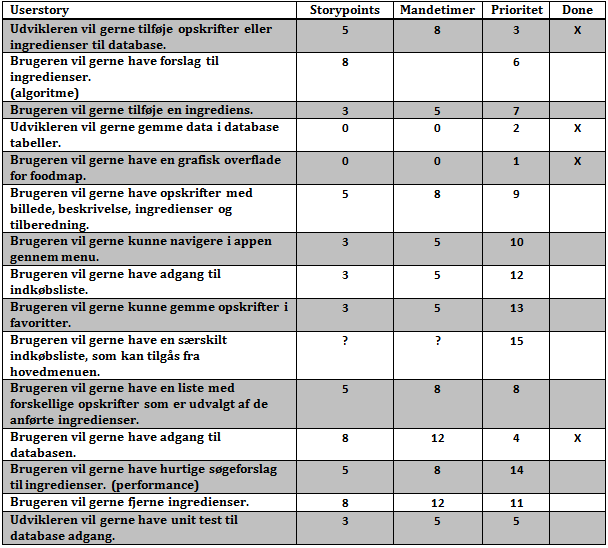
\includegraphics[scale=0.60]{includes/billeder/productbacklog_sprint3.png}

\subsubsection*{Sprint backlog}
Unit testing af database adgang og algoritme.



\subsection*{Xp og scrum praktikker}
Par programmering, simpelt design,

\subsection*{Produkt review}
Viste vores funktionalitet, samt vores unit test.

\subsubsection*{Konklusion af review}
N�ede kun unit testing.

\subsection*{Retrospektive}
Godt: \\
Vi fik lavet unit test og dermed fik vi lidt mere kvalitetssikring ind over vores projekt. \\

Kunne have v�ret bedre: \\
Alt for kort sprint med de 3 mandedage og derfor for meget pres p� for at have noget klar til reviewet. Is�r iforhold til at have noget visuelt klar at kunne vise. \\
Vi havde lidt meget parprogrammering pga. vores fokus p� test. 

Hvad �ndrer vi til n�ste sprint: \\
Vi var sprint 3 det sidste sprint, men ellers havde vi prim�rt fors�ge at lave et l�ngere sprint hvor vi arbejdede lidt mere spredt.